\documentclass[12pt, openany]{report}
\usepackage[utf8]{inputenc}
\usepackage[T1]{fontenc}
\usepackage{amsmath,amsfonts,amssymb}
\usepackage{amssymb}
\usepackage{multicol}
\usepackage[a4paper,left=2.5cm,right=2.5cm,top=2.5cm,bottom=2.5cm]{geometry}
\usepackage[english]{babel}
\usepackage{libertine}
\usepackage{graphicx}
\usepackage{wrapfig}
\usepackage{algorithm}
\usepackage{algpseudocode}
\usepackage{float}
\usepackage{enumitem}
\usepackage{pythonhighlight}
\usepackage[]{titletoc}
\usepackage{empheq}
\usepackage{titlesec}
\usepackage{mathpazo}
\usepackage{xfrac}
\usepackage{textcomp}
\usepackage{mathtools}
\usepackage{caption}
\usepackage{tabularray}
\usepackage{subcaption}
\usepackage[bottom]{footmisc}
\usepackage{pdfpages}
\usepackage{tabularx}
\usepackage {tikz}
\usetikzlibrary{positioning}
\usepackage{amsthm}
\usepackage[skins]{tcolorbox}
\titleformat{\chapter}[display]
  {\normalfont\bfseries}{}{0pt}{\Huge}
\usepackage{hyperref}
\newcommand{\hsp}{\hspace{20pt}}
\newcommand{\HRule}{\rule{\linewidth}{0.5mm}}
\newcommand{\R}{\mathbb{R}}
\newcommand{\C}{\mathbb{C}}
\newcommand{\E}{\mathbb{E}}
\theoremstyle{definition}
\newtheorem{thm}{Theorem}[chapter]
\newtheorem{definition}[thm]{Definition}
\newtheorem{lem}[thm]{Lemma}

\hbadness=100000
\begin{document}
\begin{titlepage}
    \begin{sffamily}
    \begin{center}
        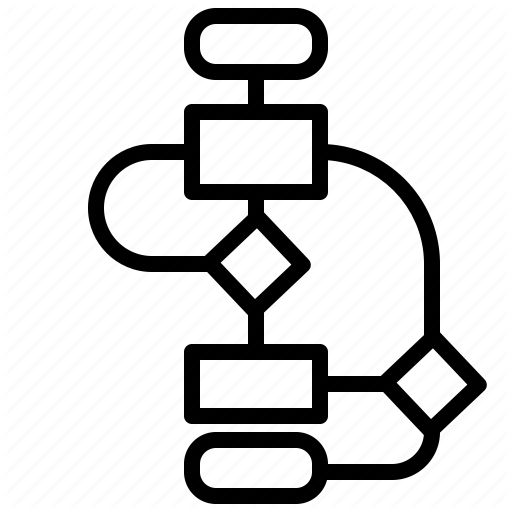
\includegraphics[scale=0.3]{img/page_de_garde.jpg} \\[1cm]
        \HRule \\[0.4cm]
        { \huge \bfseries LINMA2472 - Algorithm in data science \\[0.4cm] }
    
        \HRule \\[1.5cm]
        \textsc{\LARGE Simon Desmidt}\\[1cm]
        \vfill
        \vspace{2cm}
        {\large Academic year 2025-2026 - Q1}
        \vspace{0.4cm}
         
        
\includegraphics[width=0.15\textwidth]{img/epl.png}
        
        UCLouvain\\
    
    \end{center}
    \end{sffamily}
\end{titlepage}

\setcounter{tocdepth}{1}
\tableofcontents
\chapter{Automatic differentiation}
The Automatic differentiation is an algorithmic technique to compute automatically the derivative (gradient) of a function defined in a computer program. Unlike symbolic differentiation (done by hand) and numerical  differentiation (finite difference approximation), automatic differentiation exploits the fact that every function can be decomposed into a sequence of elementary operations (addition, multiplication, sine, exponential, etc.) and so that we can apply the chain rule to compute the derivative of the whole function. Thus we can compute the gradient of a function exactly and efficiently.\\ 
Automatic differentiation is widely used in machine learning because for the neural networks, we need to compute the gradient of a loss function with respect to the parameters of the model (weights and biases) to update them during the training process and it would be difficult to compute this manually for each node.\\
\section{Chain rule}
There is two ways to apply the chain rule to compute the gradient of a function: forward differentiation and backward differentiation. Suppose that we have a composition of $m$ functions. The chain rule gives us:
\begin{equation}
  f'(x) = f_m'(f_{m-1}(f_{m-2}(...f_1(x)...))) \cdot ... \cdot f_2'(f_1(x)) \cdot f_1'(x)
\end{equation}
Let's define:
\begin{equation}
  \begin{cases}
    s_0 &= x \\
    s_k &= f_k(s_{k-1})
  \end{cases}
\end{equation}
We thus get:
\begin{equation}
  f'(x) = f'_m(s_{m-1}) \cdot ...
  \cdot f'_2(s_1) \cdot f'_1(s_0)
\end{equation}
Based on this, we can define the forward and backward differentiation algorithms.
\section{Forward differentiation}
Also called forward mode, this algorithm consists in propagating forward the derivative and the values at the same time. It can be represented by this graph where the blue part represents the values and the green part the derivatives:
\begin{figure}[H]
    \centering
    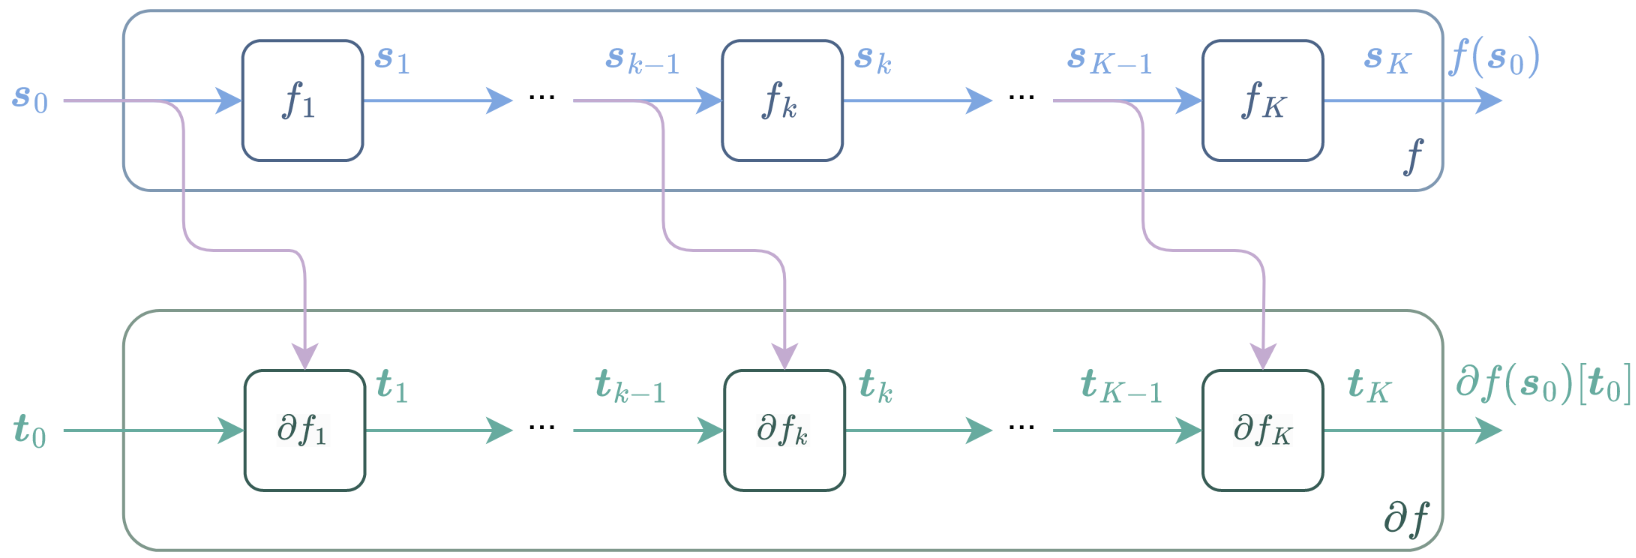
\includegraphics[width=\textwidth]{img/forward_diff.png}
    \caption{Forward differentiation}
    \label{fig:forward_diff}
\end{figure}
And it can be computed with the following recurrence relation:
\begin{equation}
  \begin{cases}
    t_0 &= 1 \\
    t_k &= f'_k(s_{k-1}) \cdot t_{k-1}\\
  \end{cases}
\end{equation}
It is simple to implement and very efficient for functions with a small number of input variables. However, it becomes inefficient for functions with a large number of input variables because we need to compute the derivative for each input variable separately. So in practice for neural networks where we have a large number of input variables (weights and biases), we use the backward differentiation.
\section{Backward differentiation}
Also called backward mode, this algorithm consists in propagating the derivative backward and the values forward at the same time. It can be represented by this graph where the blue part represents the values and the orange part the derivatives:
\begin{figure}[H]
    \centering
    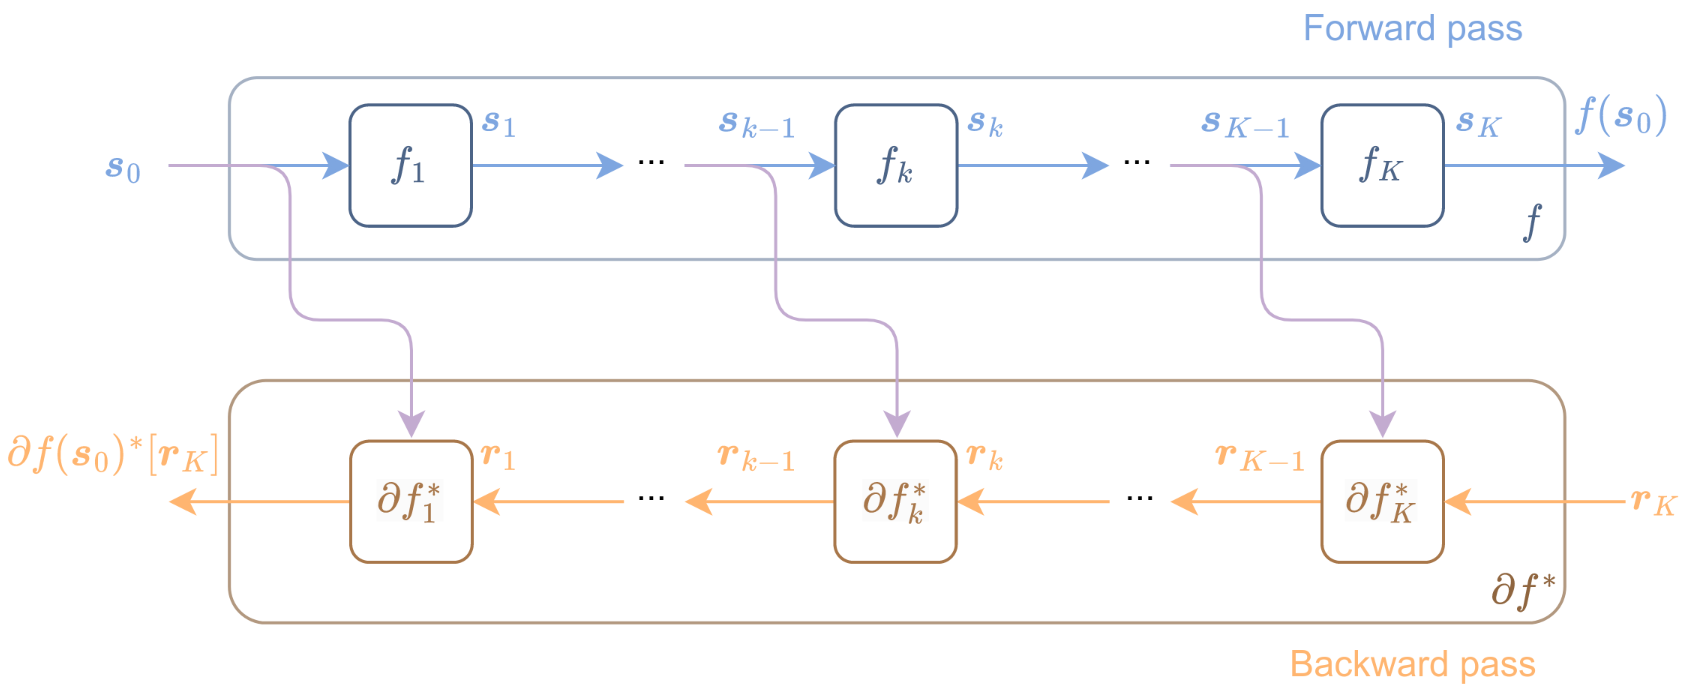
\includegraphics[width=\textwidth]{img/backward_diff.png}
    \caption{Backward differentiation}
    \label{fig:backward_diff}
\end{figure}
The idea is to compute all the intermediate values $s_k$ in a forward pass and then compute the derivatives $r_k$ based on the output in a backward pass. It can be computed with the following recurrence relation:
\begin{equation}
  \begin{cases}
    r_m &= 1 \\
    r_k &= r_{k+1} \cdot f'_{k+1}(s_{k})\\
  \end{cases}
\end{equation}
This method is more complex to implement but it is very efficient for functions with a large number of input variables and a small number of output variables typically 1, the loss function.
\section{Computational graph and multivariate differentiation}
\subsection{Computational graph}  
To represent the computation of a function, we can use a computational graph. It is a directed acyclic graph where the nodes represent the operations and the edges represent the variables. For example, consider the function with $f_1(x)=x=s_1$ and $f_2(x)=x^2=s_2$:
\begin{equation}
  f_3(s_1,s_2) = s_1 + s_2 = x + x^2
\end{equation}
The computational graph is:\\
\begin{center}
  \begin{tikzpicture}[
    roundnode/.style={circle, draw=green!60, fill=green!5, very thick, minimum size=7mm},]
    %Nodes
    \node[roundnode] (x1) {$x$};
    \node[roundnode] (square) [right=of x1] {$x^2$};
    \node[roundnode] (sum) [right=of square] {$+$};
    
    % %Lines
    \draw[->] (x1.north) .. controls +(up:7mm) and +(up:7mm).. (sum.north);
    \draw[->] (x1.east) -- (square.west);
    \draw[->] (square.east) -- (sum.west);
  \end{tikzpicture}
\end{center}
\subsection{Multivariate differentiation}
Let's consider the function of the computational graph above:
\begin{equation}
  f_3(f_1(x),f_2(x)) = f_1(x) + f_2(x) = s_1 + s_2 = x + x^2 
\end{equation}
following the chain rule, we have:
\begin{equation}
  f'_3(x) = \frac{\partial f_3}{\partial s_1} \frac{\partial s_1}{\partial x} + \frac{\partial f_3}{\partial s_2} \frac{\partial s_2}{\partial x}
\end{equation}
For the forward differentiation, we work the same way as before, we propagate the values and the derivatives forward. But when we have a node with multiple inputs, we need to use formula derivated from the chain rule. For the function $f_3$, we will have:
\begin{equation}
  \begin{cases}
    t_0 &= 1 \\
    t_1 &= f'_1(x) \cdot t_0 = 1\\
    t_2 &= f'_2(x) \cdot t_0 = 2x\\
    t_3 &= \frac{\partial f_3}{\partial s_1} \cdot t_1 + \frac{\partial f_3}{\partial s_2} \cdot t_2 = 1 + 2x\\
  \end{cases}
\end{equation}
For the backward differentiation, 
\end{document}